\documentclass[10pt]{beamer}
\usepackage[T1]{fontenc}
\usepackage[utf8]{inputenc}
\usepackage[slovene]{babel}
\usepackage{pgfpages} % privat zapiski
\usepackage{amsmath} % pravilen izpis v "math mode"
\usepackage{hyperref}
\usepackage{pgfplots}
\usepackage{tikz}
\usepackage{algorithm}
\usepackage{algorithmicx}
\usepackage{biblatex}
\addbibresource{literatura_test}

\usepackage{algpseudocode}
%\documentclass{standalone}
%\usepackage{pgfplotstable,filecontents}
\usepackage{bibentry}

\usepackage{caption}

%\addbibresource{literatura_test.bib}
\DeclareCaptionFormat{myformat}{#3}
\captionsetup[algorithm]{format = myformat}

\pgfplotsset{compat=1.8}
\hypersetup{hidelinks}
%\usetheme{Bergen}
\usecolortheme{seahorse}

\usepackage{graphicx}% http://ctan.org/pkg/graphicx
\usepackage{booktabs}% http://ctan.org/pkg/booktabs

\usepackage{palatino}
\usefonttheme{serif}

\setbeamertemplate{navigation symbols}{} % izklop navigacije
\setbeamertemplate{footline}[frame number]{} % oštevilčenje
\setbeamertemplate{note page}{\pagecolor{yellow!5}\insertnote}
\setbeamertemplate{itemize items}[circle]



\begin{document}
    \title[Diplomski seminar]{Iterativne numerične metode v posplošenih linearnih modelih}
    \author{Mitja Mandić \\ \small Mentor: izr. prof. dr. Jaka Smrekar}
    %\date{1. april 2021} 

\begin{frame}
    \titlepage
\end{frame}

\begin{frame}{Eksponentna družina}
    \begin{itemize}
        \item<1->Porazdelitev pripada enoparametrični eksponentni družini z disperzijskim parametrom, če
        ima gostoto oblike
            \begin{equation*}
            f_{Y}(y; \theta, \phi) = \exp{\left(\frac{y\theta - b(\theta)}{a(\phi)} + c(y, \phi)\right)},
        \end{equation*}
        za neke funkcije $a(\cdot), b(\cdot)\text{~in~}c(\cdot).$ Parametru $\theta$ pravimo \textit{kanonični} oziroma \textit{naravni} parameter,
        $\phi$ pa imenujemo \textit{disperzijski parameter}
        \item Velja $\mathbb{E}(Y) = b'(\theta)$ in $\mathrm{Var}(Y) = b''(\theta)a(\phi)$\pause
        \item Za $Y\sim N(\mu,\sigma^2)$ z gostoto $\tfrac{1}{\sqrt{2\pi\sigma^2}}\exp{-\tfrac{(y-\mu)^2}{2\sigma^2}}$
         izrazimo
        \[
            \theta = \mu,~\phi = \sigma^2,~a(\sigma^2)=\sigma^2,~b(\mu) = \frac{\mu^2}{2}
        \] \pause
        \item Za $Y\sim Bin(m,p)$ je $\mathrm{P}(Y = y) = \binom{m}{y}p^y(1-p)^{m-y},$ kar preoblikujemo v        \[
        \exp\left(y\log\left(\frac{p}{1-p}\right) + m\log(1-p) + \log{\binom{m}{y}}\right)
        \] in preberemo $\theta = \log\frac{p}{1-p},~b(\theta) = m\log(1 + e^{\theta}),~a(\phi) = 1.$
    \end{itemize}
\end{frame}


\begin{frame}{Posplošeni linearni modeli}    
Vsak posplošeni linearni model sestavljajo trije deli:
\begin{itemize}
    \item \alert{slučajni del} -- porazdelitev proučevane slučajne spremenljivke \pause
    \item \alert{sistematični del} -- linearna relacija med pojasnjevalnimi spremenljivkami \pause
    \item \alert{povezovalna funkcija} -- povezava med sistematičnim delom in pričakovano vrednostjo. Če je enaka naravnemu parametru
    porazdelitve ji rečemo \textit{kanonična} povezovalna funkcjia \pause
\end{itemize}
Skupaj:
\[
    g(\mu) = X\beta
\]
\end{frame}

\begin{frame}[t]
    \frametitle{Logistični model}
    \begin{itemize}
        \item<1-> Za računanje verjetnosti iz binarnih podatkov, predpostavimo model oblike
        \[
            \textrm{logit}(p) = \log\left(\frac{p}{1-p}\right) = X\beta
        \]
        \item<2->Izrazimo 
        \[
            p_{i} = \frac{\exp(x_{i}^\top\beta)}{1 + \exp(x_{i}^\top\beta)}
        \]
        \only<2>{
        \begin{figure}
            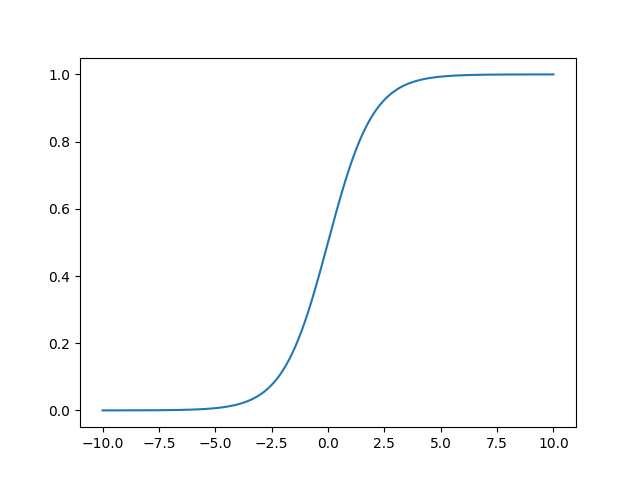
\includegraphics[width=4.5cm]{sigmoida.png}
        \end{figure}
        }
        \pause
        \item<3> Izračunamo še prvi in drugi odvod logaritemske funkcije verjetja

    \end{itemize}


\end{frame}

\begin{frame}{Metoda največjega verjetja}
    \begin{itemize}
        \item Najprej privzemimo gostote oblike $f_{X}(x;\theta) = f(x;\theta_{1},\ldots,\theta_{r})$ za nek $\theta \in \Theta^{r}$
        
        \item Pri fiksni realizaciji poskusa definiramo \textit{funkcijo verjetja}
        \[ 
            F(X_{1},\ldots,X_{n};\underbrace{\theta_{1},\ldots,\theta_{r}}_{\theta}) = f(X_{1},\theta)\cdots f(X_{n},\theta) 
        \] \pause
        \item Iščemo njen maksimum - to bo hkrati tudi maksimum $\log(F)$
        \item Sistemu 
        \[
            \frac{\partial}{\partial \theta_{j}}\log F (X,\theta) = 0,~~j=1,\ldots,r
        \]
        pravimo sistem enačb verjetja, njegova rešitev je \textit{cenilka največjega verjetja}
        \pause
        \item Niso nujno nepristranske, so pa dosledne, če je rešitev enolična
        \item \textbf{Običajno niso eksplicitno rešljive}
    \end{itemize}
\end{frame}


\begin{frame}{Numerične metode}
    \begin{itemize}
        \item 
        Iterativne metode, ki temeljijo na Newtonovi metodi za iskanje ničel funkcije
        \[
            x_{i+1} = x_{i} - \frac{f(x_{i})}{f'(x_{i})}
        \]
        \pause
        \item Za iskanje ekstremov logaritemske funkcije verjetja $\ell(\theta)$ enačimo njen gradient z nič in dobimo
        \[
            \theta_{i+1} = \theta_{i} - \frac{\frac{\partial}{\partial\theta}\ell(\theta)}{\frac{\partial^2}{\partial\theta^2}\ell(\theta)},
        \]
        računanje in invertiranje Hessiana pa je lahko problematično. Kako se lahko temu izognemo?
    \end{itemize}
    
\end{frame}

\begin{frame}{Fisherjeva zbirna metoda}
\[
    \theta_{i+1} = \theta_{i} + \mathrm{FI}(\theta)^{-1}\left(\frac{\partial}{\partial\theta}\ell\right),
\]
kjer je $\mathrm{FI}(\theta) = \mathbb{E}\left((\frac{\partial}{\partial\theta}\ell)(\frac{\partial}{\partial\theta}\ell)^\top\right)$
\pause
Informacijska enakost pravi
\begin{equation*}
    \mathrm{FI}(\theta) = \mathbb{E}\left((\frac{\partial}{\partial\theta} \ell)(\frac{\partial}{\partial\theta} \ell)^\top\right) = -\mathbb{E}\left(\frac{\partial^2}{\partial\theta^2}\ell\right),
\end{equation*}
\pause
Za kanonične povezovalne smo dokazali
\[
    \mathbb{E}\left(\frac{\partial^2}{\partial\theta^2}\ell\right) = \frac{\partial^2}{\partial\theta^2}\ell
\]
in sledi
\[
    \mathrm{FI}(\theta) = -\frac{\partial^2}{\partial\theta^2}\ell
\]
\pause
$\rightarrow$ za kanonične povezovalne funkcije Fisherjeva zbirna metoda in Newtonov algoritem sovpadata!
\end{frame}

\begin{frame}{Fisherjeva zbirna metoda}
Taylorjev polinom za funkcijo zbira (ob upoštevanju $\ell(\theta^{*}) = 0$) je
\[
    \ell(\theta^{*} + s) = \ell(\theta^{*}) + \frac{1}{2}s^\top \frac{\partial^2}{\partial\theta^2}\ell(\theta^{*})s.
\]

Poleg tega pa velja še:
\[
    -\frac{\partial^2}{\partial\theta^2}\ell = \mathrm{FI}(\theta) = \mathrm{Var}\left(\frac{\partial}{\partial\theta}\ell\right)
\]
\pause
$\rightarrow$ v $\theta^{*}$ je maksimum in imamo konstanten (naraščajoč) alogirtem!
\end{frame}

\begin{frame}{Rezultati}
    Iz interneta smo pridobili podatke o tesnilih iz vesoljskih poletov pred dobo \textit{Challengerja}
    in izračunali:
\begin{columns}
    \begin{column}{6.5cm}
    \begin{itemize}
        \item<1-> verjetnost odpovedi z logistično regresijo le s podatki o temperaturi
        \item<2-> verjetnost odpovedi s temperaturo in pritiskom
        \item<3> primerjava logistične in probit regresije le s podatki o temperaturi
    \end{itemize}
\end{column}
\begin{column}{4.5cm}
\only<1>{
    \begin{figure}
    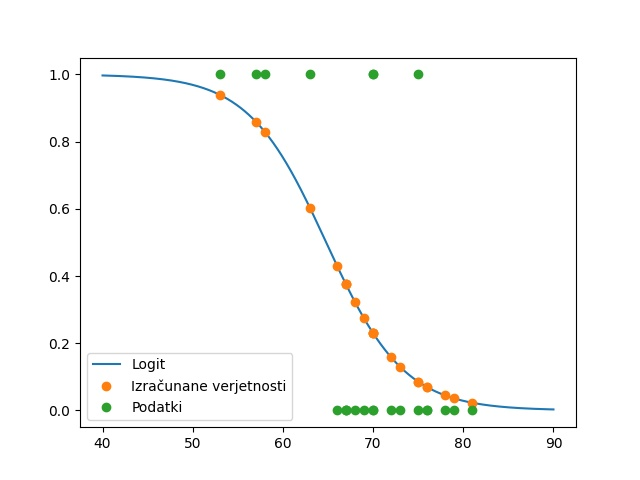
\includegraphics[width=4.5cm]{logit_challenger.jpeg}
    \end{figure}
}
\only<2>{
    \begin{figure}
        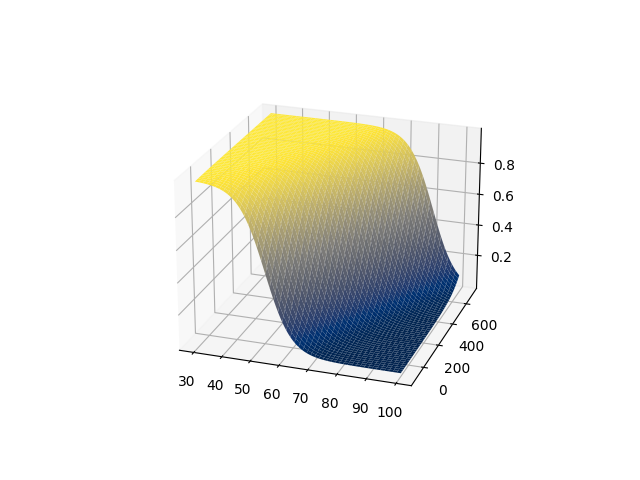
\includegraphics[width=4.5cm]{logit_3d.png}
    \end{figure}
}
\only<3>{
    \begin{figure}
        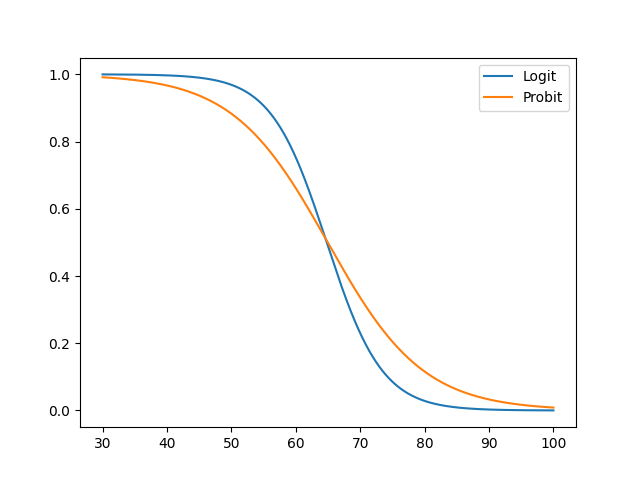
\includegraphics[width=4.5cm]{logit_probit.png}
    \end{figure}
}
\end{column}
\end{columns}
\end{frame}

\begin{frame}{Literatura}
    
\end{frame}

\end{document}